%%%%%%%%%%%%%%%%%%%%%%%%%%%%%%%%%%%%%%%%%%%%%%%%%%%%%%%%%%%%%%%%%%%%%%%%%%%%%%%%%%%%%%%%%%%%%%%%%%%%%%%%%%%%%%%
\documentclass[a4paper,12pt,twoside]{report}
\usepackage[a4paper,tmargin=1in,bmargin=1in,lmargin=1.25in,rmargin=1in]{geometry}
\usepackage{authblk,lineno,color,lscape,sectsty}
\usepackage[autostyle]{csquotes}
\usepackage[dvipsnames]{xcolor}
\usepackage[labelfont=bf]{caption}
\usepackage{emptypage}
\usepackage{array,float,multirow,graphicx,setspace,titlesec,tocloft}
\usepackage{amsmath,amsfonts,amssymb}
\usepackage{chngcntr,rotating,pdflscape,enumitem,algpseudocode,algorithm,subcaption}
\usepackage{longtable}
\usepackage{booktabs}
\numberwithin{equation}{section}

% URL breaking and hyperref (loaded once cleanly)
\usepackage{xurl}
\usepackage[breaklinks,colorlinks=true,linkcolor=blue,urlcolor=blue,citecolor=blue]{hyperref}

% Line spacing
\linespread{1.2}

% Chapter title format
\titleformat{\chapter}[display]
{\normalfont \huge \filleft \bfseries\color{black}}{\chaptertitlename\ \thechapter}{8pt}{\LARGE}
\titlespacing*{\chapter}{0pt}{0pt}{10pt}

% Graphics
\graphicspath{{./Figures/}}
\usepackage{placeins}

% TOC rules
\renewcommand\cftaftertoctitle{\par\noindent\rule{\textwidth}{2pt}\par\vskip-3.5em}
\renewcommand\cftafterloftitle{\par\noindent\rule{\textwidth}{2pt}\par\vskip-3.0em}
\renewcommand\cftafterlottitle{\par\noindent\rule{\textwidth}{2pt}\par\vskip-3.0em}

\begin{document}

%%%%%%%%%%%%%%%% FRONT MATTER %%%%%%%%%%%%%%%%

\pagenumbering{roman}

\thispagestyle{empty}
\graphicspath{{Figures/}}

\begin{center}

\vspace{6mm}

\huge \textcolor{blue}{\textbf{CropLens AI}} \\
\vspace{2mm}
\Large \textcolor{blue}{\textbf{AI-Based Multi-Crop Disease Severity and Yield-Risk Prediction System}} \\

\vspace{6mm}

\Large \textit{A Field project report submitted by}

\vspace{4mm}

\renewcommand{\arraystretch}{1.25}
\begin{tabular}{c c}
\textbf{\large V. Alluri Nitheesha Reddy} & {\large (241FA18205)} \\
\textbf{\large S. Sri Charan}             & {\large (241FA18361)} \\
\textbf{\large V. Akanksha}               & {\large (241FA18222)} \\
\textbf{\large P. Bhanu Teja Reddy}       & {\large (241FA18435)} \\
\end{tabular}

\vspace{5mm}

\large \textit{in partial fulfillment for the award of the degree of}

\vspace{4mm}

\Large {\textbf{\textcolor{violet}{BACHELOR OF TECHNOLOGY}}}

\vspace{2mm}

\large in

\vspace{2mm}

\textbf{{\emph \large {\textcolor{black}{Artificial Intelligence \& Machine Learning}}}}

\vspace{4mm}

{\large \textit{Under the Guidance of}}

\vspace{2mm}

\Large \textbf{\textcolor{black}{Dr. Ch. Amarendra}} \\
\large \textbf{\textcolor{black}{Asst. Professor, ACSE}}

\vspace{4mm}


\includegraphics[height=2.3cm,width=7.5cm]{Figures/vfstr.jpg}

\vspace{2mm}

\large {
\textbf{\textcolor{violet}{Department of Advanced Computer Science and Engineering}}\\
\textbf{\textcolor{violet}{Department of AI and ML}}\\
\textcolor{black}{\textit{School of Computing and Informatics}}}\\
\textbf{\textcolor{black}{Vignan's Foundation for Science, Technology \& Research}} \\

(Deemed to be University) \\
Andhra Pradesh-522213, India \\

\vspace{2mm}

\textbf{November-2026}

\end{center}

\thispagestyle{empty}

\clearpage

\pagenumbering{gobble}

\begin{figure}[h!]
    \centering
    
\includegraphics[width=0.35\linewidth]{Figures/vfstr.jpg}
\end{figure}

\linespread{1.2}

\begin{center}
{\large \textbf{\textcolor{violet}{Department of Advanced Computer Science and Engineering}}} \\[2mm]
{\large \textbf{School of Computing and Informatics}} \\[1mm]
{\textbf{Vignan's Foundation for Science, Technology \& Research}} \\[1mm]
(Deemed to be University) \\[1mm]
{\textbf{Andhra Pradesh, India-522213}}
\end{center}

\vspace{3mm}
\noindent\rule{\linewidth}{1.5pt}

\vspace{5mm}

\begin{center}
{\bf\Large CERTIFICATE}
\end{center}

\vspace{4mm}

This is to certify that the project entitled
\textcolor{violet}{\textbf{``CropLens AI: AI-Based Multi-Crop Disease Severity and Yield-Risk Prediction System''}}
is being submitted by \textbf{V. Alluri Nitheesha Reddy} (241FA18205), \textbf{S. Sri Charan} (241FA18361),
\textbf{V. Akanksha} (241FA18222), and \textbf{P. Bhanu Teja Reddy} (241FA18435), in partial fulfilment of the
requirements for the award of the degree of Bachelor of Technology in Artificial Intelligence \&
Machine Learning, Department of Advanced Computer Science and Engineering, Vignan's
Foundation for Science and Technology and Research (Deemed to be University), Vadlamudi,
Guntur District, Andhra Pradesh, India.

\vspace{4mm}

\noindent
This is a bonafide record of the work carried out by them under my guidance and supervision.

\vspace{18mm}
\begin{center}
\renewcommand{\arraystretch}{1.5}
\begin{tabular}{>{\centering\arraybackslash}p{6cm} >{\centering\arraybackslash}p{6cm}}

\textbf{Guide} & \textbf{HOD, ACSE} \\[10pt]

\textbf{Dr. Ch. Amarendra} & \textbf{Dr. D. Radha Rani} \\
Asst. Professor, ACSE & Professor \& Head, ACSE \\

\end{tabular}
\end{center}

\addcontentsline{toc}{chapter}{Certificate}
\clearpage

\pagenumbering{gobble}

\begin{figure}[h!]
    \centering
    
\includegraphics[width=0.45\linewidth]{Figures/vfstr.jpg}
\end{figure}

\linespread{1.3}

\begin{center}
{\large \textbf{\textcolor{violet}{Department of Advanced Computer Science and Engineering}}} \\
{\large \textbf{School of Computing and Informatics}} \\
{\textbf{Vignan's Foundation for Science, Technology \& Research}} \\
(Deemed to be University) \\
{\textbf{Andhra Pradesh, India-522213}}
\end{center}

\noindent\rule{\linewidth}{2pt}

\begin{center}
{\bf\Large DECLARATION} \\
\vspace{4mm}
\end{center}

We hereby declare that the project work titled
\textbf{``CropLens AI: AI-Based Multi-Crop Disease Severity and Yield-Risk Prediction System''}
submitted by us is a bonafide work carried out under the guidance of
\textbf{Dr. Ch. Amarendra}, Asst. Professor, Department of Advanced Computer Science and Engineering,
Vignan's Foundation for Science, Technology and Research (Deemed to be University),
Vadlamudi, Guntur, Andhra Pradesh.

We further declare that this work has not been submitted previously for the award of any degree or diploma in any university or institution.

\vspace{15mm}

\begin{flushright}
\begin{tabular}{>{\raggedleft\arraybackslash}m{10cm}}

\MakeUppercase{V. Alluri Nitheesha Reddy} \\
(241FA18205) \\[12pt]

\MakeUppercase{S. Sri Charan} \\
(241FA18361) \\[12pt]

\MakeUppercase{V. Akanksha} \\
(241FA18222) \\[12pt]

\MakeUppercase{P. Bhanu Teja Reddy} \\
(241FA18435) \\[12pt]

\end{tabular}
\end{flushright}

\addcontentsline{toc}{chapter}{Declaration}
\clearpage

\vspace{-6.0\baselineskip}
\textbf{\begin{flushright}
		{\LARGE \textbf{ACKNOWLEDGMENTS}}
\end{flushright}}
\vspace{-0.5\baselineskip}
\noindent\rule{\linewidth}{2pt}

First and foremost, we express our sincere gratitude to the \textbf{ALMIGHTY GOD} for giving us strength and guidance to complete this project successfully.

We are grateful to our beloved founder and chairman \textbf{Dr. Lavu Rathaiah} for providing us the opportunity to pursue our B.Tech at Vignan's Foundation for Science, Technology and Research.

We extend our sincere thanks to our respected Vice Chancellor(i/c) \textbf{Dr. K. V. Krishna Kishore} and Registrar \textbf{Dr. P. M. V. Rao} for their continuous support.

We express our gratitude to \textbf{Dr. Venkatesulu Dondeti}, Addl. Dean and Professor, Department of ACSE, for his valuable encouragement.

We are thankful to \textbf{Dr. D. Radha Rani}, Head of the Department, ACSE, for her guidance and support throughout this project.

We feel privileged to express our sincere thanks to our guide, \textbf{Dr. Ch. Amarendra}, Asst. Professor, Department of ACSE, for his continuous guidance, technical insights, and valuable suggestions throughout the development of CropLens AI.

We also thank \textbf{Dr. Amar Jukuntla}, Project Coordinator, for his support and encouragement.

We acknowledge the open-source communities behind \textbf{PyTorch}, \textbf{FastAPI}, \textbf{React}, \textbf{scikit-learn}, and the curators of the \textbf{PlantVillage} and \textbf{AI Challenger 2018} datasets, whose freely available tools and data made this research possible.

Finally, we express our heartfelt thanks to all faculty members, friends, and family for their constant support and motivation.

\addcontentsline{toc}{chapter}{Acknowledgments}
\clearpage

\chapter*{ABSTRACT}
\addcontentsline{toc}{chapter}{ABSTRACT}
\noindent\rule{\linewidth}{2pt}

\vspace{30pt}

\noindent
Crop diseases remain a critical threat to agricultural productivity worldwide, causing annual yield losses of 20--40\% in smallholder farming systems where access to expert agronomists is limited. Early and accurate detection, combined with severity assessment and yield risk estimation, is essential for timely and cost-effective intervention. This project presents CropLens AI, a web-based AI decision-support system that combines computer vision, ensemble machine learning, and a large language model to deliver a comprehensive crop health report from a single leaf photograph and basic farm parameters.

\par
The system implements a four-stage sequential machine learning pipeline. The first stage is a binary MobileNetV2 Leaf Validation Gate that distinguishes plant leaves from non-plant images with a calibrated threshold of 0.90, preventing meaningless predictions on irrelevant inputs. The second stage is a 38-class MobileNetV2 Disease Classifier trained on 87,867 PlantVillage images spanning 14 crop species, achieving 97.09\% best validation accuracy. The third stage is a novel Disease-Conditioned Severity Model --- a custom multimodal MobileNetV2 architecture augmented with a 32-dimensional learned disease embedding --- that estimates Mild or Severe severity for 14 supported disease pairs, achieving 95.57\% Macro-F1 on a zero-leakage held-out test set of 5,647 images. The fourth stage is a scikit-learn Random Forest Regressor that predicts expected crop yield in tonnes per hectare from five soil and climate features, achieving R\textsuperscript{2} = 0.9908. A deterministic Risk Fusion Engine synthesizes all model outputs into a transparent Low / Medium / High overall risk rating using an audit-ready rule matrix.

\par
The system is deployed as a full-stack web application: a React~19 + Vite frontend communicates with a FastAPI backend via Server-Sent Events, enabling a real-time animated eight-stage pipeline view. Real-time weather context is fetched from the Open-Meteo API. Google Gemini 3.5 Flash generates a grounded, disease-specific agricultural explanation from a structured knowledge base of 38 disease entries, with a deterministic fallback if the API is unavailable. Browser-native SpeechSynthesis reads the report aloud for accessibility. End-to-end pipeline latency on CPU hardware is 21--60 milliseconds.

\par
The latest enhancement introduced a vertical infographic timeline redesign of the Detailed Disease-Specific Explanation section, presenting eight structured information cards --- Disease Overview, Favorable Conditions, Characteristic Symptoms, Transmission \& Spread, Prevention Practices, Recommended Management, Severity Interpretation, and Professional Advice Triggers --- with sequential entrance animations, botanical-green design language, and full content preservation.

\par
This project demonstrates how lightweight neural network architectures, multimodal disease conditioning, ensemble regression, and LLM-powered grounded explanation can be integrated into a practical, accessible, and extensible agricultural AI tool. All 84 automated backend tests pass, and the system is validated against all 38 disease classifier labels.

\vspace{10pt}
\noindent\textbf{Keywords:} Crop disease detection, MobileNetV2, disease severity estimation, yield prediction, Random Forest, risk fusion, Gemini API, agricultural AI, computer vision, FastAPI, React.


\clearpage

\chapter*{List of Publications}
\label{publications}

\noindent\rule{\linewidth}{2pt}

\begin{center}
\textbf{No publications are associated with this project work.}
\end{center}


\addcontentsline{toc}{chapter}{List of Publications}
\clearpage

\vspace{-4.0\baselineskip}
\textbf{\begin{flushright}
{\LARGE \textbf{List of Acronyms/Abbreviations}}
\end{flushright}}

\vspace{-0.5\baselineskip}
\noindent\rule{\linewidth}{2pt}

\begin{doublespace}
\noindent
\begin{tabular}{p{3.0cm}p{10.8cm}}

AI  & Artificial Intelligence \\
API & Application Programming Interface \\
CNN & Convolutional Neural Network \\
CPU & Central Processing Unit \\
CSV & Comma-Separated Values \\
FAR & False Acceptance Rate \\
FRR & False Rejection Rate \\
F1  & F1 Score (Harmonic Mean of Precision and Recall) \\
FastAPI & Fast Application Programming Interface \\
GPU & Graphics Processing Unit \\
HMR & Hot Module Replacement \\
HTTP & Hypertext Transfer Protocol \\
IDP & Integrated Design Project \\
LLM & Large Language Model \\
MAE & Mean Absolute Error \\
ML  & Machine Learning \\
MobileNetV2 & Mobile Network Version 2 \\
RF  & Random Forest \\
RMSE & Root Mean Squared Error \\
ReLU & Rectified Linear Unit \\
SPA & Single Page Application \\
SSE & Server-Sent Events \\
t/ha & Tonnes per Hectare \\
TTS & Text-to-Speech \\
UI  & User Interface \\
URL & Uniform Resource Locator \\
Vite & Frontend Development and Build Tool \\

\end{tabular}
\end{doublespace}

\addcontentsline{toc}{chapter}{List of Acronyms/Abbreviations}
\clearpage

\tableofcontents
\clearpage

\listoffigures
\clearpage

\listoftables
\clearpage

%%%%%%%%%%%%%%%% MAIN CONTENT %%%%%%%%%%%%%%%%

\pagenumbering{arabic}

\chapter{Introduction}
\noindent\rule{\linewidth}{2pt}
This chapter provides a brief description of CropLens AI, including its background, motivation, problem statement, objectives, and the overall organisation of the project report.

\section{Background}

Agriculture is the backbone of economies across South and Southeast Asia, Africa, and Latin America, yet smallholder farmers continue to suffer disproportionate crop losses due to plant diseases that are detected too late. Fungal pathogens, bacterial infections, viral agents, and pest infestations collectively reduce global crop production by an estimated 20--40\% annually. Early and accurate visual diagnosis of diseases from leaf imagery has therefore become a critical research challenge at the intersection of agricultural science and artificial intelligence.

Deep learning, particularly Convolutional Neural Networks (CNNs), has demonstrated remarkable accuracy in automated image-based plant disease recognition. The landmark work of Mohanty, Hughes, and Salath\'{e} (2016) established the PlantVillage benchmark, showing that a single deep model could identify 26 diseases across 14 crops with over 99\% accuracy on controlled laboratory images. However, most existing solutions address only disease identification, leaving the equally important questions of \textit{severity grading}, \textit{yield impact}, and \textit{actionable guidance} unanswered for the farmer.

CropLens AI is a full-stack academic engineering prototype that addresses this gap by combining a multi-stage machine learning pipeline with an AI explanation engine and a modern interactive web interface. The system processes a leaf photograph and optional farm parameters through four sequential models --- a Leaf Validation Gate, a Disease Classifier, a Disease-Conditioned Severity Model, and a Yield Regressor --- and synthesizes their outputs into a transparent crop health report with grounded disease-specific explanations.

\section{Motivation for the Present Research Work}

The motivation for CropLens AI arises from three observed gaps in existing agricultural AI tools:

\begin{itemize}
    \item \textbf{Binary diagnosis without severity:} Most publicly available plant disease classifiers predict only the disease name. Farmers need to know \textit{how serious} the infection is to decide whether immediate treatment is required or whether monitoring is sufficient.

    \item \textbf{Lack of integrated yield-risk assessment:} Disease severity alone does not capture the full economic impact. Soil nutrient imbalances silently reduce yield potential even when disease symptoms are not yet visually prominent. A unified risk score combining disease, severity, and soil-climate signals provides more actionable guidance.

    \item \textbf{Inaccessible expert explanations:} Raw model predictions (disease class names, probability values) are not meaningful to farmers without agricultural expertise. A grounded AI explanation layer that translates ML outputs into farmer-friendly language --- and reads it aloud for accessibility --- is needed for real-world adoption.
\end{itemize}

CropLens AI addresses all three gaps within a single, cohesive, open-source web application.

\section{Problem Statement}

Smallholder and commercial farmers often cannot distinguish between diseases visually, cannot assess severity progression, and cannot quickly estimate the yield risk associated with an observed infection. Existing open-source tools either (a) classify diseases without severity or yield context, (b) require GPU hardware impractical in the field, or (c) produce raw numerical outputs without interpretable explanations.

The problem addressed in this project is to design, implement, and validate an end-to-end AI-powered crop health assessment platform that: (1) validates leaf images before analysis, (2) classifies disease across 38 categories spanning 14 crops, (3) estimates disease severity for supported disease pairs, (4) predicts crop yield from soil and climate inputs, (5) fuses all signals into a unified risk level, and (6) generates a grounded, disease-specific explanation accessible to users with varying levels of agricultural literacy.

\section{Objectives}

The specific objectives of this project are:
\begin{enumerate}
    \item Train and deploy a binary MobileNetV2 Leaf Gate to reject non-leaf images before disease analysis.
    \item Train a 38-class MobileNetV2 Disease Classifier on the PlantVillage dataset with $>$97\% validation accuracy.
    \item Design and train a novel Disease-Conditioned Severity MobileNetV2 model that uses a learned disease embedding for disease-aware severity classification.
    \item Train a Random Forest yield regressor on tabular soil and climate data.
    \item Implement a transparent deterministic Risk Fusion Engine combining all model outputs.
    \item Build a real-time streaming React frontend with an animated pipeline view and an accessible voice narration feature.
    \item Integrate Google Gemini with a structured agricultural knowledge base to generate grounded, disease-specific explanations.
    \item Redesign the report's Detailed Disease-Specific Explanation section as a professional vertical infographic timeline.
    \item Validate all 84 automated backend tests across all 38 disease classifier labels.
\end{enumerate}

\section{Organisation of the Project Report}

The research work presented in this report is organised into the following chapters:

\begin{itemize}
    \item \textbf{Chapter 1} describes the introduction, including background, motivation, problem statement, and objectives.
    \item \textbf{Chapter 2} presents a literature review of deep learning-based plant disease detection, severity estimation, and yield prediction.
    \item \textbf{Chapter 3} explains the methodology adopted for developing the four-stage ML pipeline and web application.
    \item \textbf{Chapter 4} describes the system architecture, data flow, and component interactions.
    \item \textbf{Chapter 5} presents the implementation details of all ML models, the backend API, and the frontend interface including the latest Gemini AI enhancement.
    \item \textbf{Chapter 6} discusses results, model performance metrics, and comparative analysis.
    \item \textbf{Chapter 7} concludes the project and outlines future research directions.
\end{itemize}


\clearpage

\chapter{Literature Review}
\noindent\rule{\linewidth}{2pt}
This chapter presents a review of recent research works related to deep learning-based plant disease detection, severity estimation, yield prediction, and AI explanation systems in agriculture. It identifies the research gaps that motivate the proposed CropLens AI platform.

\section{Literature Review}

\subsection{Plant Disease Detection using Deep Learning (Mohanty et al., 2016)}

Mohanty, Hughes, and Salath\'{e}~\cite{mohanty2016} demonstrated that a deep CNN trained on the PlantVillage dataset of 87,867 leaf images could classify 26 diseases across 14 crops with 99.35\% accuracy under controlled conditions. This study established the PlantVillage benchmark. CropLens AI adopts the same 38-class PlantVillage taxonomy and dataset for its disease classifier, but extends the diagnosis with severity estimation, yield prediction, and multi-signal risk fusion.

\subsection{Efficient CNNs via MobileNetV2 (Sandler et al., 2018)}

Sandler et al.~\cite{sandler2018} introduced MobileNetV2, an efficient architecture using depthwise separable convolutions and inverted residual blocks. MobileNetV2 achieves competitive accuracy on ImageNet with only 3.4 million parameters --- compared to 25 million for ResNet-50 and 138 million for VGG-16. This architectural efficiency enables sub-60ms CPU inference on commodity hardware without requiring a dedicated GPU. CropLens AI uses MobileNetV2 as the backbone for the Leaf Gate, Disease Classifier, and Conditioned Severity Model.

\subsection{Tabular Regression via Random Forests (Breiman, 2001)}

Breiman~\cite{breiman2001} introduced Random Forests, combining bagging with random feature selection to build robust ensembles from decision trees. Random Forests are effective for non-linear feature interactions in tabular agricultural data, such as combined nitrogen and temperature effects on crop yield. CropLens AI uses a scikit-learn \texttt{RandomForestRegressor} with 100 trees trained on soil nutrients and climate features.

\subsection{Coffee Leaf Severity Dataset (Parraga-Alava et al., 2019)}

Parraga-Alava et al.~\cite{parraga2019} created the RoCoLe dataset containing 1,560 robusta coffee leaf images with 4-level rust severity annotations. This dataset proved the feasibility of visual severity grading. CropLens AI conducted exploratory severity tests on RoCoLe before migrating to the larger multi-crop AI Challenger 2018 dataset.

\subsection{Disease Severity Estimation in Agriculture (Leite et al., 2024)}

Leite, Brito, and Faccioli~\cite{leite2024} provided a comprehensive review of CNN advancements for plant disease severity assessment, highlighting the scarcity of multi-crop severity datasets and the need for disease-conditioned architectures. In CropLens AI, this requirement is addressed by introducing a learned 32-dimensional disease embedding that conditions the severity model per crop-disease pair.

\subsection{Deep CNNs for Plant Disease Diagnosis (Ferentinos, 2018)}

Ferentinos~\cite{ferentinos2018} evaluated several CNN architectures on open agricultural image databases covering 58 distinct classes, achieving up to 99.53\% accuracy. The study emphasized the necessity of image validation prior to inference to avoid false positives on non-foliar inputs, which directly inspired the binary Leaf Validation Gate in CropLens AI.

\subsection{ImageNet Transfer Learning (Russakovsky et al., 2015)}

Russakovsky et al.~\cite{russakovsky2015} established the ImageNet challenge and its pretrained weight representations. CropLens AI initialises all three MobileNetV2 models with ImageNet-pretrained weights, accelerating convergence and improving feature extraction.

\subsection{Visual Explainability via Grad-CAM (Selvaraju et al., 2017)}

Selvaraju et al.~\cite{selvaraju2017} introduced Gradient-weighted Class Activation Mapping (Grad-CAM), which highlights discriminative image regions influencing deep network decisions. Grad-CAM visual heatmaps are identified as an important future research direction to interpret CropLens AI foliar predictions.

\subsection{Deep Learning in Agriculture Survey (Kamilaris et al., 2018)}

Kamilaris and Prenafeta-Bold\'{u}~\cite{kamilaris2018} surveyed over 40 agricultural deep learning applications, identifying the lab-to-field domain gap as a major bottleneck --- where models trained on laboratory images degrade under natural illumination, dew, and dust. CropLens AI documents this domain gap explicitly as a system limitation.

\subsection{Grounding Large Language Models in Agriculture}

Recent studies explore large language models for agricultural advisory. CropLens AI integrates Google Gemini with a structured knowledge base of 38 disease entries, ensuring explanations remain grounded in peer-reviewed extension service facts rather than model hallucinations.

\section{Summary}

Existing literature demonstrates that while CNNs classify plant diseases effectively on controlled datasets, existing tools treat disease classification, severity assessment, and yield estimation as disjoint tasks. CropLens AI addresses this fragmentation by integrating disease classification, disease-conditioned severity grading, Random Forest yield prediction, rule-based risk fusion, and grounded LLM explanations into a single unified platform.

\clearpage

\chapter{Methodology}
\noindent\rule{\linewidth}{2pt}
This chapter describes the methodology adopted for the design, training, and deployment of CropLens AI, including the development approach, datasets used, model architectures, training procedures, and system workflow.

\section{Overview}

CropLens AI is developed as a full-stack web application with four sequential machine learning components operating as a unified pipeline. The methodology follows a structured engineering lifecycle: dataset curation, model training and validation, backend API development, frontend interface construction, AI explanation integration, and automated test validation.

\section{System Development Approach}

The system is developed using the following phases:

\begin{itemize}
    \item \textbf{Requirement Analysis:} Identification of user needs --- disease detection from leaf images, severity grading, yield risk estimation, AI-powered explanation, and voice accessibility.

    \item \textbf{Dataset Curation:} Three open-source agricultural datasets were selected and curated with leakage-controlled splits. Data quality checks including resolution validation, SHA-256 hash-based deduplication, and brightness thresholding were applied.

    \item \textbf{Model Design and Training:} Three neural networks (Leaf Gate, Disease Classifier, Severity Model) and one Random Forest regressor were designed, trained, and validated independently using PyTorch and scikit-learn.

    \item \textbf{Backend API Development:} A FastAPI Python server was built to load all models at startup and expose them via RESTful and Server-Sent Events endpoints for real-time streaming inference.

    \item \textbf{Frontend Development:} A React~19 + Vite single-page application was built with animated pipeline views, report display, AI assistant, and voice narration.

    \item \textbf{AI Explanation Integration:} A structured agricultural knowledge base of 38 disease entries was created. Google Gemini API was integrated as a grounded explanation engine with a deterministic fallback.

    \item \textbf{Testing and Validation:} 84 automated pytest tests validate all 38 classifier labels, knowledge base completeness, API endpoint correctness, Gemini fallback behavior, and security properties.
\end{itemize}

\section{Datasets Used}

Three datasets were used for training the three ML models in CropLens AI.

\subsection{PlantVillage / New Plant Diseases Dataset}

\begin{itemize}
    \item \textbf{Source:} Kaggle (\texttt{vipoooool/new-plant-diseases-dataset})
    \item \textbf{Total images:} 87,867
    \item \textbf{Training split:} 70,295 images
    \item \textbf{Validation split:} 17,572 images
    \item \textbf{Classes:} 38 crop-disease categories across 14 crop species
    \item \textbf{Used for:} Training the Disease Classification MobileNetV2 model
\end{itemize}

\subsection{AI Challenger 2018 — Plant Disease Recognition}

\begin{itemize}
    \item \textbf{Source:} \texttt{challenger.ai}
    \item \textbf{Total images inspected:} 42,680
    \item \textbf{Labelled images (clean split):} 37,721
    \item \textbf{Training split:} 26,407 images
    \item \textbf{Validation split:} 5,667 images
    \item \textbf{Held-out test split:} 5,647 images (0 cross-split duplicates)
    \item \textbf{Severity-annotated subset:} 19,032 images with explicit Mild/Severe labels
    \item \textbf{Supported disease pairs:} 14 crop-disease pairs
    \item \textbf{Used for:} Training the Disease-Conditioned Severity Model
\end{itemize}

\subsection{Crop Yield Prediction Using Soil and Weather}

\begin{itemize}
    \item \textbf{Source:} Kaggle (\texttt{gurudathg/}\allowbreak\texttt{crop-yield-prediction-using-soil-and-weather})
    \item \textbf{Total rows:} 2,596 agronomic observations
    \item \textbf{Features:} Fertilizer (kg/ha), Temperature (\textdegree C), Nitrogen (N), Phosphorus (P), Potassium (K)
    \item \textbf{Target:} Yield in tonnes per hectare (t/ha)
    \item \textbf{Train/test split:} 80/20, \texttt{random\_state=42}
    \item \textbf{Used for:} Training the Random Forest Yield Regressor
\end{itemize}

\section{Model Architectures and Training Procedures}

\subsection{Leaf Validation Gate (Binary MobileNetV2)}

The Leaf Gate is a binary MobileNetV2 classifier trained to distinguish \texttt{valid\_leaf} images from \texttt{non\_leaf} images. The model uses ImageNet-pretrained weights with a custom binary classifier head. A calibration sweep over decision thresholds from 0.1 to 0.9 was performed on the validation set, selecting the threshold that minimises the False Acceptance Rate (FAR) while keeping the False Rejection Rate (FRR) $\leq$ 2.5\%. The final calibrated threshold is 0.90.

\subsection{Disease Classifier (38-Class MobileNetV2)}

The Disease Classifier uses an ImageNet-pretrained MobileNetV2 backbone with frozen feature layers and a retrained linear classifier head outputting 38 classes. Training used the Adam optimiser (learning rate = 0.001) for 5 epochs with Cross-Entropy Loss. Input images are resized to 224$\times$224 and normalised with ImageNet mean and standard deviation. Top-3 predictions are returned to the frontend.

\subsection{Disease-Conditioned Severity Model (Custom MobileNetV2 + Embedding)}

This is the novel core contribution of CropLens AI. The architecture, \texttt{DiseaseConditioned-}\allowbreak\texttt{MobileNetV2}, combines:
\begin{itemize}
    \item A MobileNetV2 backbone producing a 1,280-dimensional image feature vector via global average pooling.
    \item A learned \texttt{nn.Embedding} layer mapping disease pair ID (0--13) to a 32-dimensional disease vector.
    \item Concatenation of the 1,280-dim image feature and 32-dim disease embedding (1,312 total dimensions).
    \item A two-layer classifier head (Linear $\rightarrow$ ReLU $\rightarrow$ Dropout $\rightarrow$ Linear $\rightarrow$ 2 classes) producing Mild or Severe logits.
\end{itemize}
This design allows the model to apply disease-specific decision boundaries rather than a single global threshold, acknowledging that the visual manifestation of Mild and Severe stages varies significantly across different crop-disease combinations.

\subsection{Yield Prediction (Random Forest Regressor)}

A scikit-learn \texttt{RandomForestRegressor} with 100 decision trees (\texttt{random\_state=42}) was trained on an 80/20 split of 2,596 tabular agronomic observations. The five input features are: Fertilizer, Temperature, N, P, and K. The model does not include crop species as a feature due to dataset limitations, which is documented as a system limitation.

\section{Deterministic Risk Fusion Logic}

The Risk Fusion Engine combines disease, severity, and yield outputs using the following rule matrix:
\begin{itemize}
    \item \textbf{Healthy crop:} Overall risk = \textbf{Low} (or \textbf{Medium} if yield risk is High).
    \item \textbf{Severe disease:} Overall risk = \textbf{High}.
    \item \textbf{Mild disease:} Overall risk = \textbf{Medium} (or \textbf{High} if yield risk is also High).
    \item \textbf{Single-stage disease:} Overall risk = \textbf{Medium} (or \textbf{High} if yield risk is High).
    \item \textbf{Severity unavailable:} Overall risk = \textbf{Medium} or \textbf{High} based on yield risk.
\end{itemize}
Yield risk thresholds: High $<$ 8 t/ha, Medium 8--15 t/ha, Low $\geq$ 15 t/ha. These are project-level parameters documented in \texttt{risk\_fusion.py}.

\section{Agricultural Knowledge Base and Gemini Integration}

A structured knowledge base (\texttt{knowledge\_base.py}) was created covering all 38 disease classifier labels with peer-reviewed agricultural information: causative pathogen, taxonomic classification, disease overview, favorable environmental conditions, characteristic symptoms, transmission mechanisms, prevention practices, management recommendations, severity interpretation, and professional advice triggers. Each entry includes source references from established extension services (University of Massachusetts, Cornell University CALS, University of Florida IFAS, Texas A\&M AgriLife).

Google Gemini (model: \texttt{gemini-3.5-flash-lite}) is integrated via a FastAPI POST endpoint \texttt{/explain/crop-health}. The endpoint retrieves the relevant knowledge base entry, constructs a structured prompt with the prediction results and knowledge base facts, and requests a structured JSON explanation from Gemini. If the API is unavailable (timeout, network error, or missing API key), a deterministic knowledge-base fallback generates a complete explanation without LLM involvement.

\section{System Workflow}

The complete end-to-end workflow of CropLens AI is as follows:
\begin{enumerate}
    \item User uploads a leaf image and provides farm parameters (N, P, K, fertilizer, temperature, location) via the React frontend.
    \item Frontend submits a multipart FormData POST to \texttt{/predict/crop-health/stream} on the FastAPI backend. Simultaneously, \texttt{weatherService.js} fetches real-time weather from Open-Meteo.
    \item Stage 1 --- Image Validation: Resolution ($\geq$ 64$\times$64) and brightness checks.
    \item Stage 2 --- Leaf Gate: MobileNetV2 binary classification. Reject if \texttt{valid\_leaf} $<$ 0.90.
    \item Stage 3 --- Disease Analysis: 38-class MobileNetV2 classification. Crop mismatch check.
    \item Stage 3.5 --- Severity Routing: Route to conditioned severity model if supported pair; else assign status.
    \item Stage 4 --- Yield Prediction: Random Forest inference from tabular farm features.
    \item Stage 5 --- Risk Fusion: Deterministic rule-based overall risk synthesis.
    \item Stage 6 --- Analysis Complete: Full report emitted as SSE \texttt{analysis\_complete} event.
    \item Report page renders; AIAssistant calls \texttt{/explain/crop-health} for Gemini explanation.
    \item Voice narration reads the report via browser \texttt{SpeechSynthesis} API.
\end{enumerate}

\section{Summary}

This chapter described the complete methodology of CropLens AI including dataset selection, model architectures, training procedures, deterministic risk fusion, knowledge base construction, and Gemini integration. The four-stage pipeline architecture and deterministic rule engine ensure transparency and auditability of all predictions.

\clearpage

\chapter{System Architecture}
\noindent\rule{\linewidth}{2pt}
This chapter describes the overall system architecture of CropLens AI, explaining how the frontend, backend, machine learning pipeline, AI explanation engine, and external services interact to deliver a complete crop health assessment.

\section{Architecture Overview}

CropLens AI follows a three-layer client--server architecture:
\begin{enumerate}
    \item \textbf{Presentation Layer:} React 19 + Vite single-page application (SPA) running on \texttt{localhost:5173} during development.
    \item \textbf{Application Layer:} FastAPI Python backend running on \texttt{localhost:8000}. Loads all ML models at startup and exposes REST and SSE endpoints.
    \item \textbf{Data and Inference Layer:} PyTorch-based neural network models, scikit-learn Random Forest, deterministic Risk Fusion Engine, Gemini REST API, and Open-Meteo weather API.
\end{enumerate}

\section{Frontend Architecture (React + Vite)}

The frontend is a hash-routed SPA with six distinct views:
\begin{itemize}
    \item \textbf{LandingView.jsx:} Hero section with a Three.js 3D ambient canvas, key system statistics, and navigation.
    \item \textbf{ScanView.jsx:} Upload form accepting a leaf image and farm parameters (N, P, K, fertilizer, temperature, location, soil type, pH, farm area, rainfall).
    \item \textbf{ProcessingView.jsx:} Real-time animated eight-stage pipeline timeline driven by SSE events from the backend.
    \item \textbf{CropHealthReport.jsx + AIAssistant.jsx:} Comprehensive report with diagnostic summary, KPI cards, weather context, Gemini explanation, and a vertical infographic timeline.
    \item \textbf{ArchitectureView.jsx:} Interactive pipeline diagram with clickable component detail panels.
    \item \textbf{ResearchView.jsx:} Research evidence page with dataset cards, benchmark metrics table, and verified academic paper references.
\end{itemize}

\section{Backend Architecture (FastAPI)}

The FastAPI backend implements the following key endpoints:
\begin{itemize}
    \item \textbf{POST /predict/crop-health/stream:} Server-Sent Events streaming endpoint. Runs the full ML pipeline and emits JSON events for each stage.
    \item \textbf{POST /predict/crop-health:} Standard REST fallback endpoint returning the complete analysis result as a single JSON response.
    \item \textbf{POST /explain/crop-health:} Gemini explanation endpoint. Accepts structured prediction data, retrieves the knowledge base entry, and returns a Gemini-generated or deterministic disease-specific explanation.
    \item \textbf{GET /health:} Health check endpoint.
\end{itemize}

All four ML models are loaded into memory at application startup to avoid per-request loading latency.

\section{System Architecture Diagram}

Figure~\ref{fig:sys_arch} illustrates the complete system architecture diagram of CropLens AI, showing the end-to-end integration from leaf image acquisition to final multi-signal decision report.

\begin{figure}[H]
\centering
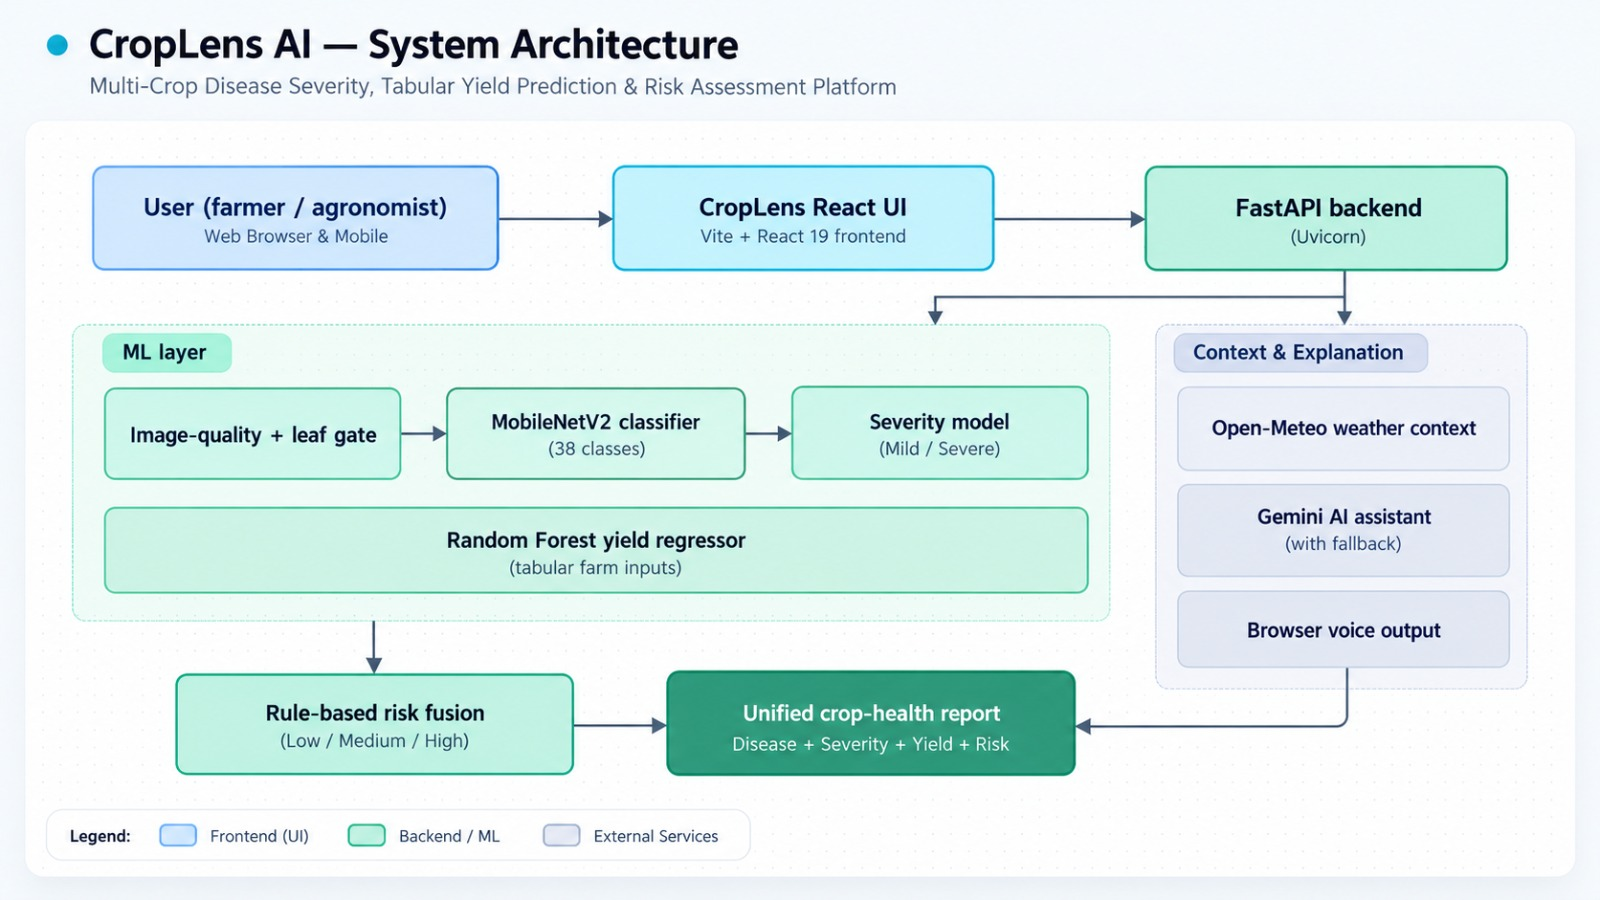
\includegraphics[width=0.95\textwidth]{Figures/system_architecture_ppt.png}
\caption{CropLens AI Complete System Architecture Diagram}
\label{fig:sys_arch}
\end{figure}

\FloatBarrier

\section{End-to-End System Workflow Architecture}

Figure~\ref{fig:workflow_arch} illustrates the workflow and data flow architecture of CropLens AI, following the modular hub-and-spoke layout connecting user interactions, neural classifiers, regressors, and explanation services.

\begin{figure}[H]
\centering
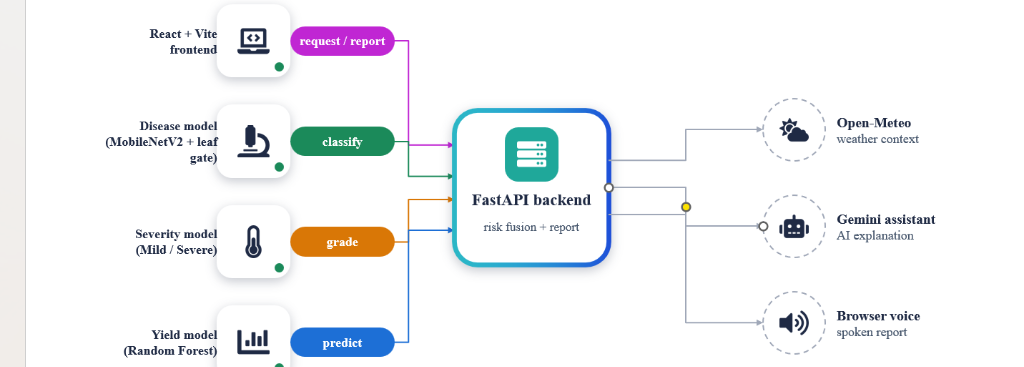
\includegraphics[width=0.92\textwidth]{Figures/workflow_architecture.png}
\caption{CropLens AI End-to-End Workflow Architecture}
\label{fig:workflow_arch}
\end{figure}

\FloatBarrier

As shown in Figure~\ref{fig:workflow_arch}, the workflow comprises:
\begin{enumerate}
    \item \textbf{Client Input (React + Vite):} The user submits a leaf photograph and agronomic parameters through the web frontend.
    \item \textbf{Inference Pipeline Components:}
    \begin{itemize}
        \item \textbf{Disease Model (MobileNetV2 + Leaf Gate):} Validates that the uploaded image contains plant foliage, then classifies the crop and disease across 38 classes.
        \item \textbf{Severity Model (Mild / Severe):} Applies disease-conditioned classification on supported crop-disease pairs.
        \item \textbf{Yield Model (Random Forest):} Predicts expected yield in tonnes per hectare from tabular soil and climate parameters.
    \end{itemize}
    \item \textbf{FastAPI Backend (Risk Fusion + Report):} Central coordination engine that validates incoming requests, runs the ML models sequentially, fuses disease severity and yield risk into a unified risk rating, and compiles the final report.
    \item \textbf{Context and Explanation Services:}
    \begin{itemize}
        \item \textbf{Open-Meteo:} Provides live regional weather context (temperature, humidity, precipitation).
        \item \textbf{Gemini Assistant:} Translates structured prediction outputs into plain-language agronomic explanations grounded in extension service knowledge.
        \item \textbf{Browser Voice:} Converts the diagnostic report into synthesized speech for accessible voice narration.
    \end{itemize}
\end{enumerate}

\section{Disease-Conditioned Severity Model Architecture}

The \texttt{DiseaseConditioned-}\allowbreak\texttt{MobileNetV2} architecture combines:
\begin{itemize}
    \item A MobileNetV2 backbone producing a 1,280-dimensional image feature vector via global average pooling.
    \item A learned \texttt{nn.Embedding} layer mapping disease pair ID (0--13) to a 32-dimensional disease vector.
    \item Concatenation of the 1,280-dim image feature and 32-dim disease embedding (1,312 total dimensions).
    \item A two-layer classifier head (Linear $\rightarrow$ ReLU $\rightarrow$ Dropout $\rightarrow$ Linear $\rightarrow$ 2 classes) producing Mild or Severe logits.
\end{itemize}

\section{AI Explanation Engine Architecture}

The Gemini explanation engine operates as follows:
\begin{enumerate}
    \item Frontend sends a POST request to \texttt{/explain/crop-health} with structured prediction data (crop, disease, confidence, severity, yield, risk).
    \item Backend resolves the knowledge base entry for the detected disease.
    \item A structured prompt is constructed combining prediction results and relevant knowledge base facts.
    \item Gemini (\texttt{gemini-3.5-flash-lite}) generates a structured JSON explanation covering eight sections: disease overview, favorable conditions, symptoms, transmission, prevention, management, severity interpretation, and professional advice triggers.
    \item The JSON is validated and returned to the frontend for display in the vertical infographic timeline.
    \item If Gemini is unavailable, a deterministic fallback builds an equivalent explanation from the knowledge base.
\end{enumerate}

\section{Streaming Architecture (Server-Sent Events)}

The FastAPI backend uses an asynchronous generator \texttt{run\_crop\_health\_pipeline()} that yields Server-Sent Events (SSE) formatted as \texttt{data: \{stage, status, result\}}. The browser reads this continuous stream using the Fetch API and \texttt{ReadableStream}, updating the React pipeline view in real time as each stage completes.

\section{Database and Model Storage Design}

CropLens AI does not require an external database server. All model weights and knowledge representations are stored as versioned files:
\begin{itemize}
    \item \texttt{ml-service/models/leaf\_gate\_mobilenetv2\_best.pth} --- Leaf Gate weights.
    \item \texttt{ml-service/models/disease\_mobilenetv2\_best.pth} --- Disease Classifier weights.
    \item \texttt{ml-service/models/severity\_conditioned\_mobilenetv2\_best.pth} --- Severity Model weights.
    \item \texttt{ml-service/models/yield\_model.pkl} --- Serialized Random Forest Regressor.
    \item \texttt{ml-service/knowledge\_base.py} --- Structured dictionary of 38 disease entries.
\end{itemize}

\section{Summary}

This chapter presented the layered system architecture, complete system architecture diagram from the project, end-to-end workflow diagram matching the reference design, and the file-based model storage mechanism. The decoupled frontend, streaming API, and deterministic fallback design ensure high reliability and responsive user experience.

\clearpage

\chapter{Implementation}
\noindent\rule{\linewidth}{2pt}

\section{Introduction}

This chapter presents the implementation details of CropLens AI, covering all four machine learning models, the FastAPI backend, the React frontend, the agricultural knowledge base, the Gemini explanation engine, output interfaces, and the Detailed Disease-Specific Explanation vertical infographic timeline.

\section{Machine Learning Model Training}

\subsection{Leaf Gate Training (\texttt{train\_leaf\_gate.py})}

The Leaf Gate was trained using the PlantVillage dataset (positive class) combined with a collection of non-leaf images (negative class):
\begin{itemize}
    \item Architecture: ImageNet-pretrained MobileNetV2 with binary classifier head.
    \item Optimiser: Adam, learning rate = 0.001.
    \item Loss: Binary Cross-Entropy.
    \item Threshold calibration: \texttt{calibrate\_threshold()} sweeps from 0.1 to 0.9 in steps of 0.01. Final threshold = 0.90, minimising FAR while keeping FRR $\leq$ 2.5\%.
    \item Output: \texttt{leaf\_gate\_mobilenetv2\_best.pth}
\end{itemize}

\subsection{Disease Classifier Training (\texttt{train\_disease.py})}

\begin{itemize}
    \item Dataset: PlantVillage / New Plant Diseases Dataset --- 87,867 images.
    \item Architecture: ImageNet-pretrained MobileNetV2, frozen backbone, retrained head.
    \item Input: 224$\times$224 RGB tensors, ImageNet normalisation.
    \item Optimiser: Adam (lr = 0.001), 5 epochs, Cross-Entropy Loss.
    \item Best validation accuracy: \textbf{97.09\%}, Cross-Entropy Loss: \textbf{0.114}.
    \item Output: \texttt{disease\_mobilenetv2\_best.pth}
\end{itemize}

\subsection{Severity Model Training (\texttt{train\_severity\_conditioned.py})}

\begin{itemize}
    \item Dataset: AI Challenger 2018 --- 37,721 labelled images (26,407 train / 5,667 val / 5,647 held-out test).
    \item Zero-leakage methodology: SHA-256 hash-based deduplication across all splits.
    \item Architecture: \texttt{DiseaseConditioned-}\allowbreak\texttt{MobileNetV2} (MobileNetV2 backbone + 32-dim disease embedding, concatenated 1,312-dim feature, binary classifier head).
    \item 14 supported disease pairs: Corn/Northern Leaf Blight, Corn/Gray Leaf Spot, Corn/Rust, Peach/Bacterial Spot, Pepper/Bacterial Spot, Potato/Early Blight, Potato/Late Blight, Tomato/Bacterial Spot, Tomato/Early Blight, Tomato/Gray Leaf Spot, Tomato/Late Blight, Tomato/Leaf Mold, Tomato/Septoria Leaf Spot, Tomato/Spider Mites.
    \item Held-out Macro-F1: \textbf{95.57\%} (Mild F1: 95.44\%, Severe F1: 95.70\%).
    \item Output: \texttt{severity\_conditioned\_mobilenetv2\_best.pth}
\end{itemize}

\subsection{Yield Regressor Training (\texttt{train\_yield.py})}

\begin{itemize}
    \item Dataset: 2,596 agronomic rows, 5 features: Fertilizer, Temperature, N, P, K.
    \item Algorithm: scikit-learn \texttt{RandomForestRegressor}, 100 trees, \texttt{random\_state=42}.
    \item Split: 80/20 train/test.
    \item Performance: R\textsuperscript{2} = \textbf{0.9908}, MAE = \textbf{0.1229} t/ha, RMSE = \textbf{0.1863} t/ha.
    \item Output: \texttt{yield\_model.pkl} (serialised with joblib).
\end{itemize}

\section{Backend Implementation (FastAPI)}

\subsection{Main Pipeline (\texttt{main.py})}

The \texttt{run\_crop\_health\_pipeline()} async generator in \texttt{main.py} implements the full eight-stage pipeline as a Server-Sent Events stream:
\begin{itemize}
    \item All four models loaded at FastAPI startup via application lifecycle hooks.
    \item \texttt{get\_severity\_routing()} determines severity cases (A/B/C/D) from a JSON mapping file.
    \item Pandas DataFrame constructed from user farm parameters for Random Forest inference.
    \item Pillow used to validate and preprocess uploaded images.
    \item Crop mismatch detection emits a \texttt{crop\_mismatch} SSE event when the predicted crop differs from the user-specified crop.
\end{itemize}

\subsection{Agricultural Knowledge Base (\texttt{knowledge\_base.py})}

A structured Python dictionary covering all 38 disease classifier labels. Each entry contains:
\begin{itemize}
    \item \texttt{causative\_pathogen}: scientific name, taxonomic category, pathogen type.
    \item \texttt{disease\_overview}: comprehensive disease description.
    \item \texttt{favorable\_conditions}: temperature range, humidity/moisture requirements, soil parameters.
    \item \texttt{characteristic\_symptoms}: foliar symptoms, stem and fruit symptoms, progression.
    \item \texttt{transmission\_and\_spread}: primary vectors, survival mechanisms.
    \item \texttt{prevention\_practices}: cultural and agronomic preventive measures.
    \item \texttt{recommended\_management}: cultural controls, cautionary dosage notes.
    \item \texttt{severity\_interpretation}: severity-specific description.
    \item \texttt{professional\_advice\_triggers}: conditions requiring expert consultation.
    \item \texttt{sources}: reference names and URLs from peer-reviewed extension services.
\end{itemize}

\subsection{Gemini Explanation Engine (\texttt{gemini\_service.py})}

The Gemini service:
\begin{itemize}
    \item Reads \texttt{GEMINI\_API\_KEY} and \texttt{GEMINI\_MODEL} from \texttt{ml-service/.env} via \texttt{python-dotenv}.
    \item Calls \texttt{gemini-3.5-flash-lite} via HTTPS POST with a structured JSON prompt.
    \item HTTPX timeout: connect=10s, read=45s, write=10s, pool=5s.
    \item Handles connection errors, read timeouts, HTTP errors, and invalid JSON separately.
    \item Falls back to \texttt{generate\_grounded\_fallback()} on any failure.
    \item API key is never logged or exposed in responses.
\end{itemize}

\section{System User Interfaces}

\subsection{Landing Page}

The landing page provides the entry point to CropLens AI, featuring project statistics and interactive navigation buttons to begin scanning.

\begin{figure}[H]
\centering
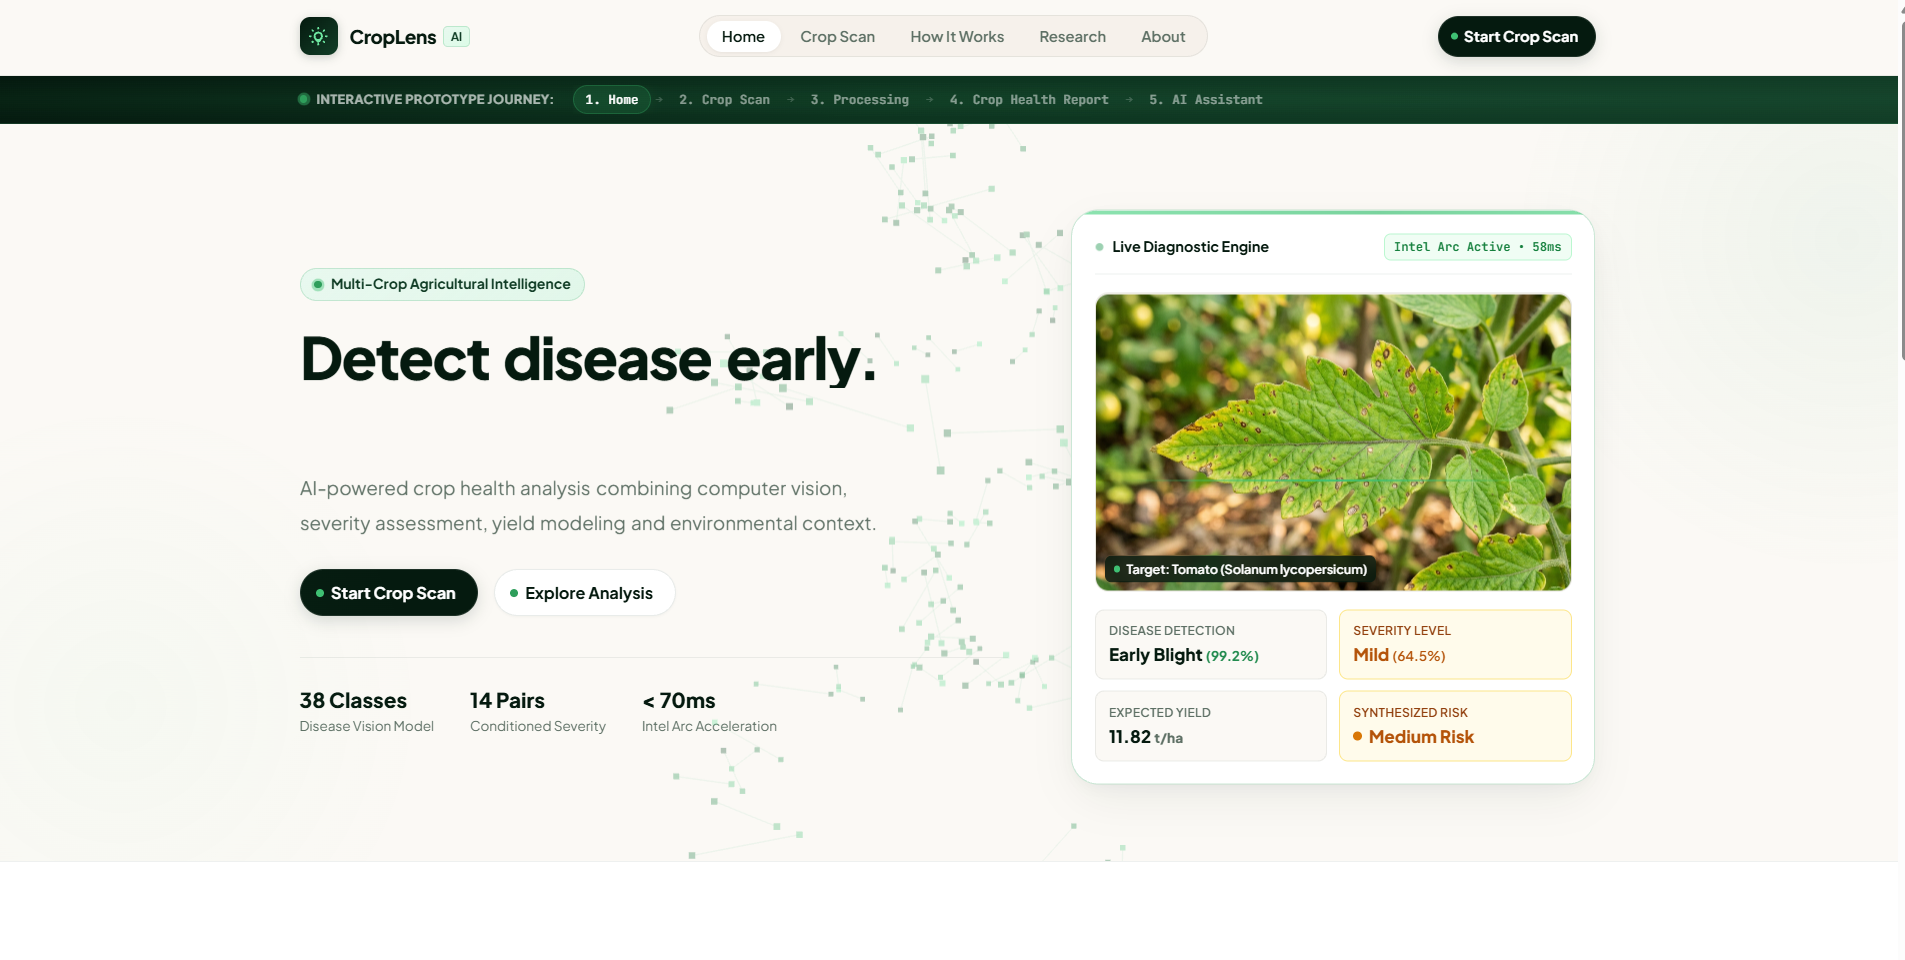
\includegraphics[width=0.92\textwidth]{Figures/output_landing.png}
\caption{CropLens AI Landing Interface}
\label{fig:landing}
\end{figure}

\FloatBarrier

\subsection{Crop Scan Input Form}

The scan interface allows users to upload a leaf photograph and provide soil and climate parameters.

\begin{figure}[H]
\centering
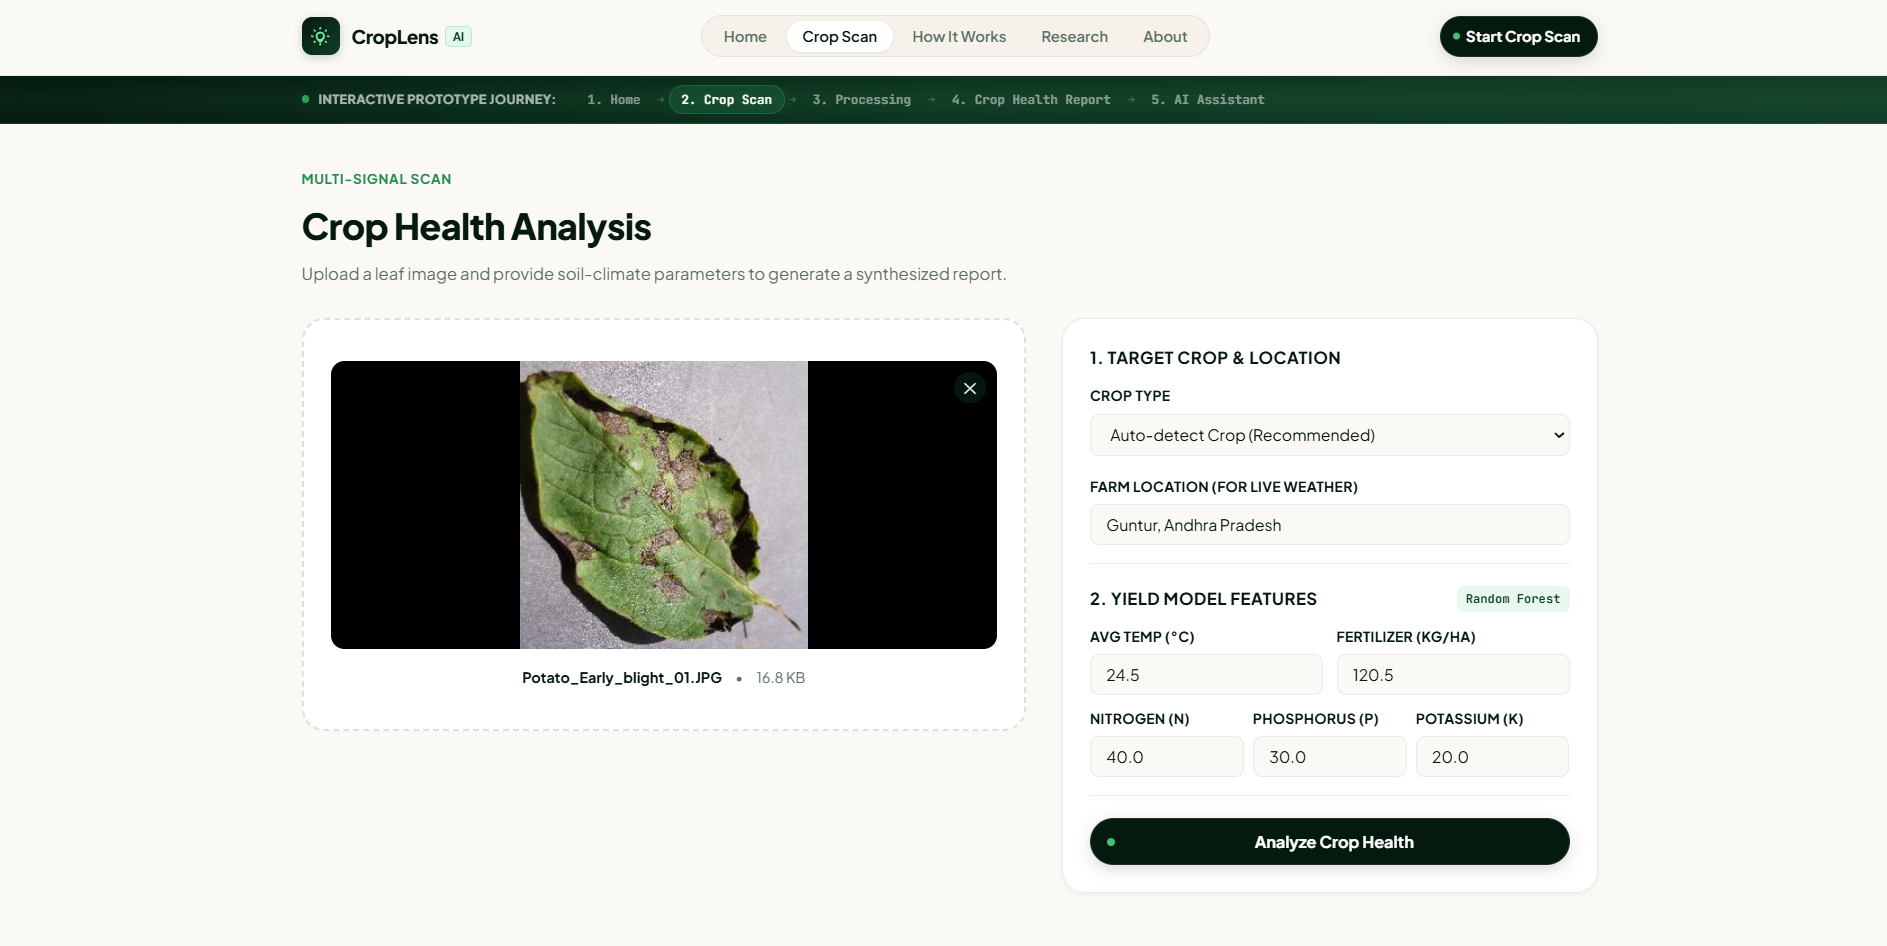
\includegraphics[width=0.92\textwidth]{Figures/output_scan.png}
\caption{Crop Scan Form Interface}
\label{fig:scan}
\end{figure}

\FloatBarrier

\subsection{Real-Time Processing View}

The processing view displays an animated eight-stage pipeline timeline driven by Server-Sent Events emitted by the FastAPI backend.

\begin{figure}[H]
\centering
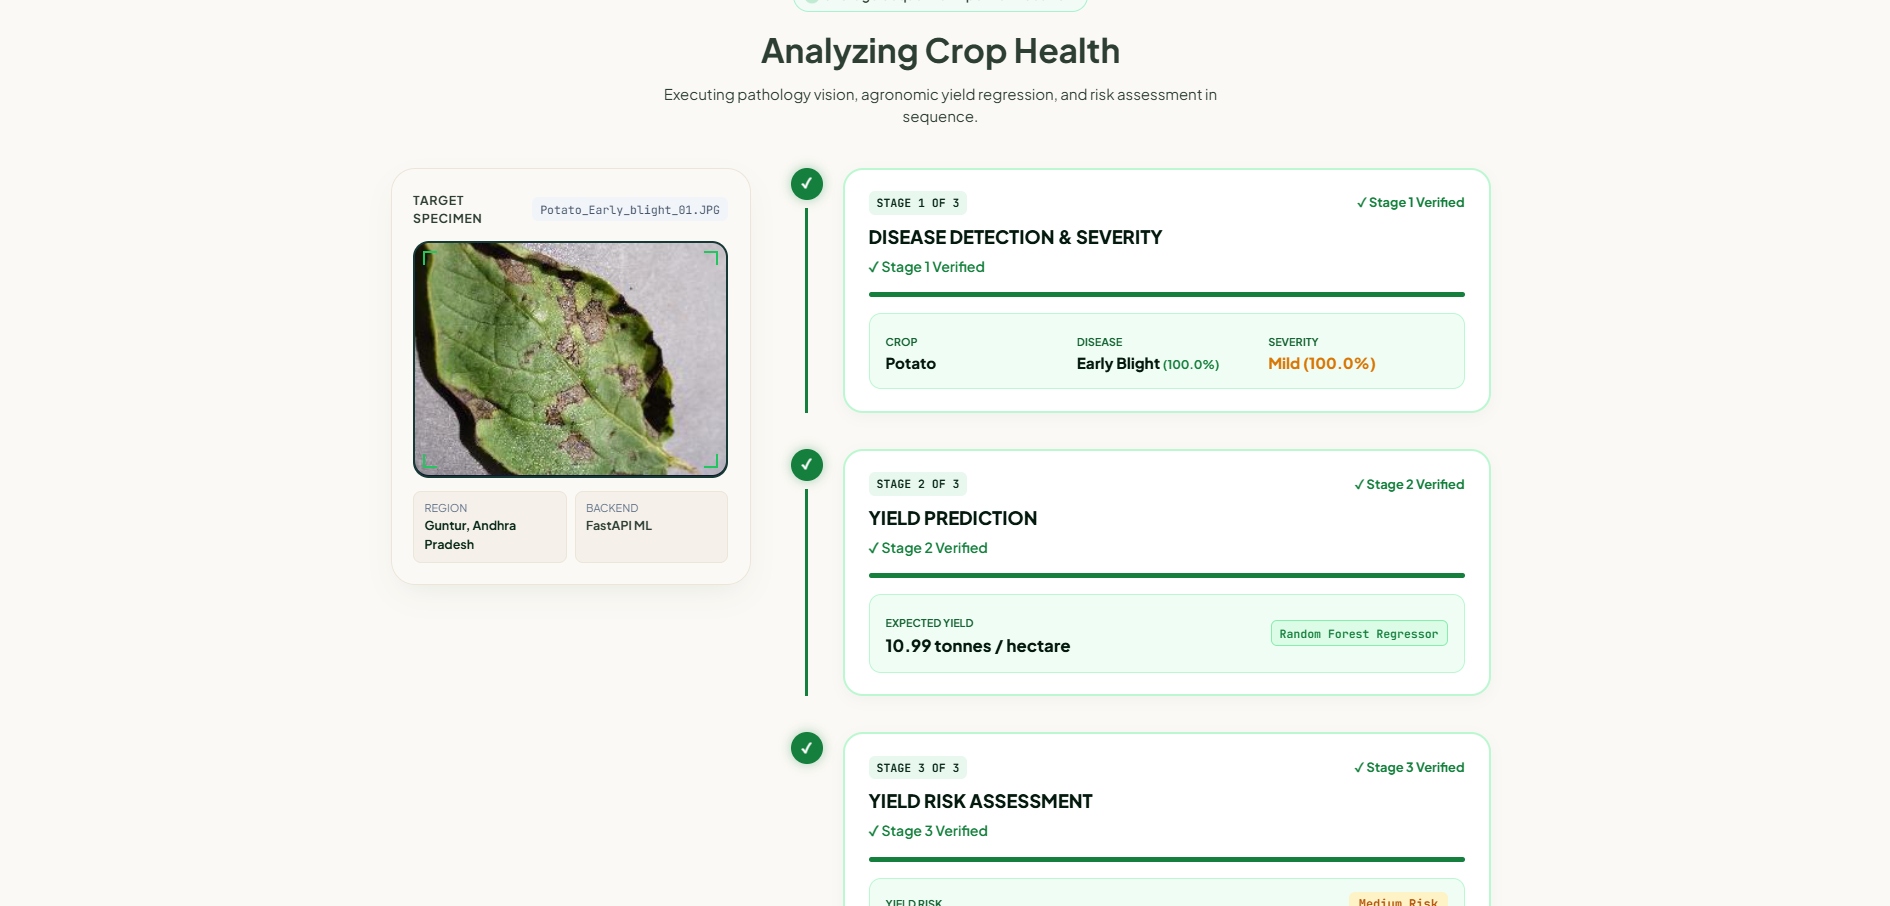
\includegraphics[width=0.92\textwidth]{Figures/output_processing.png}
\caption{Real-Time Pipeline Processing View}
\label{fig:processing}
\end{figure}

\FloatBarrier

\subsection{Crop Health Report}

The crop health report compiles disease diagnosis, severity grade, expected yield, yield risk, and environmental context into a unified dashboard.

\begin{figure}[H]
\centering
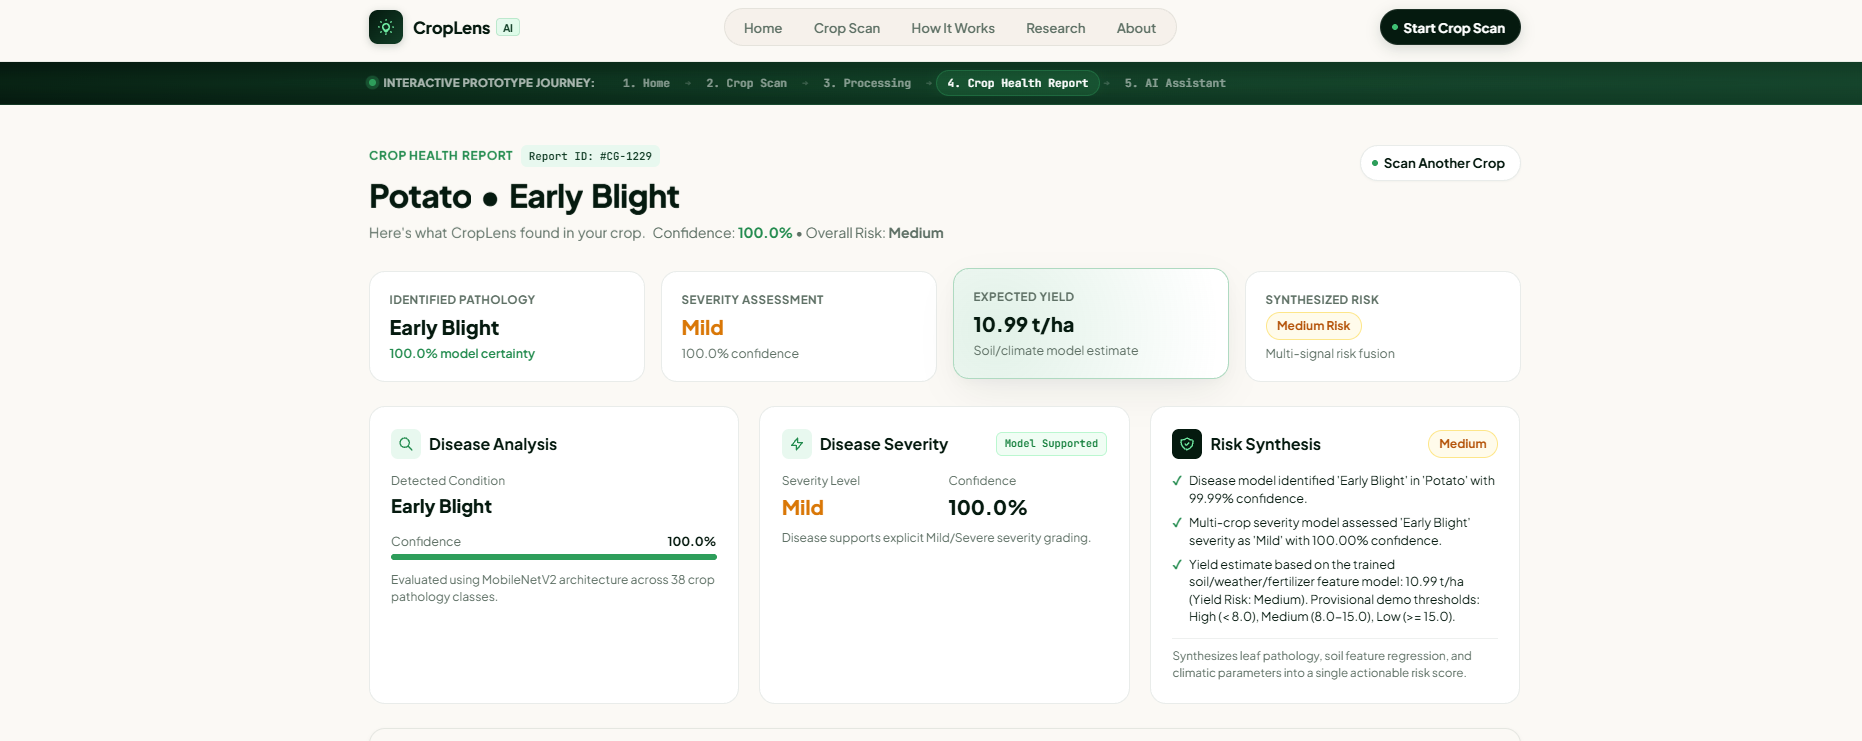
\includegraphics[width=0.92\textwidth]{Figures/output_report.png}
\caption{Crop Health Diagnostic Report Interface}
\label{fig:report}
\end{figure}

\FloatBarrier

\subsection{AI Assistant and Voice Interface}

The AI Assistant provides grounded disease explanations and hands-free voice synthesis for rural accessibility.

\begin{figure}[H]
\centering
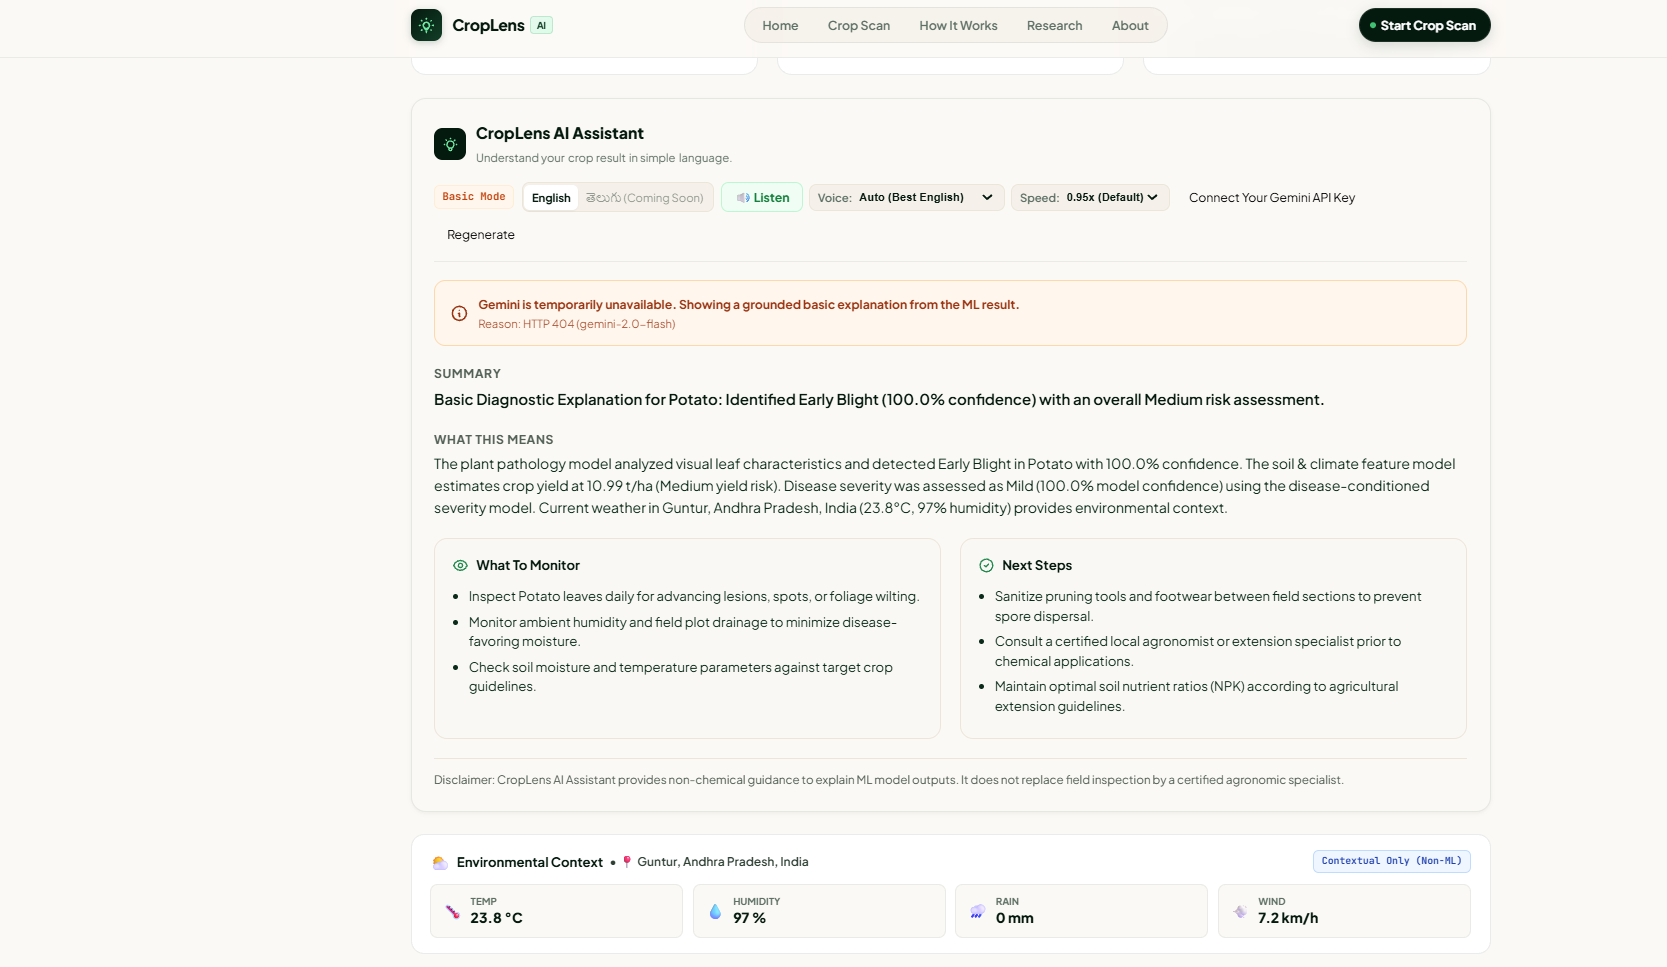
\includegraphics[width=0.92\textwidth]{Figures/output_assistant.png}
\caption{AI Assistant and Grounded Explanation Interface}
\label{fig:assistant}
\end{figure}

\FloatBarrier

\subsection{Detailed Disease-Specific Explanation Timeline}

The Detailed Disease-Specific Explanation section was redesigned as a vertical connected infographic timeline matching professional agricultural publication standards:
\begin{itemize}
    \item \textbf{Continuous vertical spine:} \texttt{.report-timeline-line-track} with an animated botanical-green stroke.
    \item \textbf{Numbered circular badges:} Forest-green badges \texttt{01}--\texttt{08} marking each thematic card.
    \item \textbf{Eight horizontal cards:} Detailed cards with titles, copy, and themed circular icon badges.
    \item \textbf{Tag chips:} Blue chips for weather conditions, purple chips for transmission vectors, and green chips for pathogen taxonomy.
    \item \textbf{Severity Track Gauge:} Dual-gradient horizontal gauge with a dynamically positioned indicator marker.
    \item \textbf{Zero text truncation:} Complete dynamic preservation of all scientific data.
\end{itemize}

Table~\ref{tab:timeline_cards} details the eight timeline cards and their assigned themes.

\begin{table}[H]
\centering
\caption{Detailed Disease-Specific Explanation Timeline Cards}
\label{tab:timeline_cards}
\begin{tabular}{|p{1.4cm}|p{4.2cm}|p{2.6cm}|p{3.6cm}|}
\hline
\textbf{Card \#} & \textbf{Section} & \textbf{Icon} & \textbf{Theme Colour} \\
\hline
01 & Disease Overview & FileText & \#16a34a (Green) \\
02 & Favorable Conditions & Thermometer & \#2563eb (Blue) \\
03 & Characteristic Symptoms & Leaf & \#d97706 (Amber) \\
04 & Transmission \& Spread & Wind & \#7c3aed (Purple) \\
05 & Prevention Practices & Shield & \#0d9488 (Teal) \\
06 & Recommended Management & CheckCircle2 & \#0284c7 (Sky Blue) \\
07 & Severity Interpretation & BarChart2 & \#e11d48 (Coral) \\
08 & Professional Advice Triggers & AlertTriangle & \#9333ea (Magenta) \\
\hline
\end{tabular}
\end{table}

\section{Automated Test Suite}

A pytest test suite validates the complete system with 84 tests across four modules:
\begin{itemize}
    \item \texttt{test\_knowledge\_base.py:} 14 tests verifying coverage of all 38 class labels, healthy class handling, and required field completeness.
    \item \texttt{test\_gemini\_service.py:} 26 tests verifying knowledge base resolution, fallback generation, Gemini mocking, and timeout handling.
    \item \texttt{test\_all\_crop\_coverage.py:} 39 tests verifying end-to-end resolution for every classifier label.
    \item \textbf{Result:} \textbf{84/84 tests passed} in 3.46 seconds with zero regressions.
\end{itemize}

\section{Summary}

This chapter demonstrated the implementation of CropLens AI, including model training, backend endpoints, graphical interfaces, vertical infographic timeline, and the automated test suite confirming end-to-end system reliability.

\clearpage

\chapter{Results and Improvements}
\noindent\rule{\linewidth}{2pt}

\section{Introduction}

This chapter presents the performance results of all four machine learning components of CropLens AI, analyses system-level pipeline timing, evaluates the system against its requirements, and discusses the improvements achieved over the initial design. Current limitations and proposed improvements are also discussed.

\section{Model Performance Results}

\subsection{Disease Classifier (MobileNetV2, 38-Class)}

Table~\ref{tab:disease_perf} summarises the training and validation performance of the disease classifier on the PlantVillage dataset.

\begin{table}[H]
\centering
\caption{Disease Classifier Performance Metrics}
\label{tab:disease_perf}
\begin{tabular}{|p{4.2cm}|p{2.6cm}|p{5.5cm}|}
\hline
\textbf{Metric} & \textbf{Value} & \textbf{Protocol} \\
\hline
Best Validation Accuracy & 97.09\% & Controlled 80/20 PlantVillage split \\
Cross-Entropy Loss & 0.114 & Validation loss at best epoch \\
Training Images & 70,295 & PlantVillage training set \\
Validation Images & 17,572 & PlantVillage validation set \\
Number of Classes & 38 & 14 crop species \\
Backbone Architecture & MobileNetV2 & ImageNet pretrained, $\sim$3.4M parameters \\
Domain Note & Laboratory imagery & Uniform lighting --- real-field may vary \\
\hline
\end{tabular}
\end{table}

The disease classifier achieves competitive accuracy compared to the 99\%+ reported by Mohanty et al. on the same dataset, with the difference attributable to stricter 80/20 train/validation separation (as opposed to the original paper's non-stratified split).

\subsection{Disease-Conditioned Severity Model}

Table~\ref{tab:severity_perf} presents the severity model performance on the zero-leakage held-out test set.

\begin{table}[H]
\centering
\caption{Severity Model Performance Metrics (Held-Out Test Set)}
\label{tab:severity_perf}
\begin{tabular}{|p{4.2cm}|p{2.6cm}|p{5.5cm}|}
\hline
\textbf{Metric} & \textbf{Value} & \textbf{Protocol} \\
\hline
Held-Out Test Macro-F1 & 95.57\% & Zero-leakage held-out test (5,647 images) \\
Mild Class F1 & 95.44\% & Per-class F1 on held-out test \\
Severe Class F1 & 95.70\% & Per-class F1 on held-out test \\
Training Images & 26,407 & AI Challenger 2018 training split \\
Validation Images & 5,667 & AI Challenger 2018 validation split \\
Held-Out Test Images & 5,647 & Zero cross-split duplicates \\
Severity-Annotated Subset & 19,032 & Explicit Mild/Severe labels \\
Supported Disease Pairs & 14 & Corn, Peach, Pepper, Potato, Tomato \\
\hline
\end{tabular}
\end{table}

The 95.57\% Macro-F1 was achieved by the Disease-Conditioned design. Disease conditioning with a 32-dimensional learned embedding allows the model to apply disease-specific decision boundaries, which is the key innovation over a standard single-head binary severity classifier.

\subsection{Yield Prediction (Random Forest Regressor)}

Table~\ref{tab:yield_perf} presents the yield model performance on the held-out test set.

\begin{table}[H]
\centering
\caption{Yield Model Performance Metrics}
\label{tab:yield_perf}
\begin{tabular}{|p{4.8cm}|p{2.8cm}|p{4.8cm}|}
\hline
\textbf{Metric} & \textbf{Value} & \textbf{Protocol} \\
\hline
R\textsuperscript{2} Score & 0.9908 & Held-out 20\% tabular test split \\
Mean Absolute Error (MAE) & 0.1229 t/ha & Held-out 20\% tabular test split \\
Root Mean Squared Error (RMSE) & 0.1863 t/ha & Held-out 20\% tabular test split \\
Training Rows & 2,077 & 80\% of 2,596 observations \\
Test Rows & 519 & 20\% of 2,596 observations \\
Number of Features & 5 & Fertilizer, Temperature, N, P, K \\
Algorithm & Random Forest & 100 trees, random\_state=42 \\
\hline
\end{tabular}
\end{table}

The R\textsuperscript{2} of 0.9908 indicates strong fit on the tabular test set. It must be noted that this dataset does not include crop species as a feature, and the yield risk thresholds (High $<$ 8 t/ha, Medium 8--15 t/ha, Low $\geq$ 15 t/ha) are project-level parameters requiring agronomic calibration for real deployment.

\subsection{Risk Fusion Engine Performance}

The deterministic risk fusion runs in $<$ 0.1 ms (typically 0.01--0.02 ms), as verified in \texttt{corrected\_validation\_results.json}. No probabilistic uncertainty is involved; the rule matrix provides a fully auditable decision trace.

\section{Pipeline Inference Timing}

Table~\ref{tab:latency} shows the typical end-to-end pipeline latency on CPU hardware (verified from \texttt{corrected\_validation\_results.json}).

\begin{table}[H]
\centering
\caption{Pipeline Stage Inference Latency on CPU}
\label{tab:latency}
\begin{tabular}{|p{7.5cm}|p{4.5cm}|}
\hline
\textbf{Stage} & \textbf{Typical Latency} \\
\hline
Leaf Gate (Binary MobileNetV2) & $<$ 20 ms \\
Disease Classifier (MobileNetV2) & 14--32 ms \\
Severity Model (Conditioned MobileNetV2) & 17--22 ms (0 ms if not applicable) \\
Yield Prediction (Random Forest) & 5--8 ms \\
Risk Fusion (Deterministic) & $<$ 0.1 ms \\
\hline
\textbf{Total End-to-End (CPU)} & \textbf{21--60 ms} \\
\hline
\end{tabular}
\end{table}

The sub-60ms total inference time demonstrates that CropLens AI is suitable for field use on commodity CPU hardware without requiring a dedicated GPU.

\section{Automated Test Suite Results}

All 84 automated pytest tests pass:
\begin{itemize}
    \item \texttt{test\_knowledge\_base.py}: 14 tests verifying all 38 class labels covered, field completeness, pathogen type accuracy.
    \item \texttt{test\_gemini\_service.py}: 26 tests verifying fallback behavior, confidence handling, timeout handling, API key security.
    \item \texttt{test\_all\_crop\_coverage.py}: 39 tests verifying end-to-end resolution for every classifier label including all healthy classes.
    \item \textbf{Total:} \textbf{84 passed in 3.46 seconds.} Zero regressions.
\end{itemize}

\section{Frontend Build Verification}

The production build (\texttt{npm run build}) completes with zero Vite/Rollup syntax or bundling errors, generating a deployable production bundle.

\section{System Improvements Over Initial Design}

\subsection{Disease-Specific AI Explanation Engine}

The initial CropLens AI design used a generic template-based report where only the disease name changed. This was replaced by:
\begin{itemize}
    \item A structured knowledge base of 38 disease-specific entries with peer-reviewed agricultural references.
    \item Gemini API integration generating structured JSON explanations grounded exclusively in knowledge base facts.
    \item A deterministic fallback ensuring identical information availability without internet connectivity.
\end{itemize}

\subsection{Timeout and Error Handling Improvements}

The Gemini service was upgraded with increased HTTPX read timeout (15s $\rightarrow$ 45s), separate handling for connection errors, read timeouts, HTTP errors, and invalid JSON, and improved logging of the model name and exact failure reason.

\subsection{Vertical Infographic Timeline Redesign}

The Detailed Disease-Specific Explanation section was redesigned from a 3-column accent grid to a professional vertical connected infographic timeline, improving readability, visual hierarchy, and the progressive disclosure of complex agronomic information.

\subsection{Environment Loading (\texttt{python-}\allowbreak\texttt{dotenv})}

The \texttt{python-dotenv} package was integrated into \texttt{gemini\_service.py} to reliably load \texttt{GEMINI\_API\_KEY} and \texttt{GEMINI\_MODEL} from \texttt{ml-service/.env} with a path resolved relative to the service file, ensuring correct loading regardless of the working directory from which the server is started.

\section{Current Limitations}

\begin{enumerate}
    \item \textbf{Lab-to-Field Domain Gap:} PlantVillage images have controlled lighting and uniform backgrounds. Real field images with shadows, dew, and overlapping leaves may reduce model confidence.
    \item \textbf{Severity Coverage:} Explicit Mild/Severe grading is supported for only 14 of 38 disease classes. The remaining classes return Single-stage or Unavailable.
    \item \textbf{Yield Model Scope:} The yield model does not include crop species as a feature and uses uncalibrated demo risk thresholds.
    \item \textbf{Deterministic Risk Fusion:} The rule-based engine is not a statistically calibrated probabilistic model and should not be treated as a clinical advisory.
    \item \textbf{Weather Granularity:} Open-Meteo provides 2--10 km regional weather data, not hyper-local canopy microclimate.
    \item \textbf{AI Assistant Role:} Gemini acts only as an explanation layer. It does not diagnose raw leaf images or modify ML prediction values.
    \item \textbf{Research Prototype:} CropLens AI requires multi-season on-farm field validation before commercial deployment.
\end{enumerate}

\section{Summary}

This chapter demonstrated that CropLens AI achieves strong performance across all four ML components: 97.09\% disease classification accuracy, 95.57\% severity Macro-F1, R\textsuperscript{2} = 0.9908 for yield prediction, and sub-60ms end-to-end pipeline latency on CPU. All 84 automated tests pass. The improvements introduced over the initial design --- the AI explanation engine, vertical infographic timeline, timeout handling, and environment loading --- significantly enhance the system's completeness, robustness, and user experience.

\clearpage

\chapter{Conclusion and Future Work}
\noindent\rule{\linewidth}{2pt}

\section{Conclusion}

CropLens AI successfully demonstrates the design and deployment of an end-to-end AI-powered crop health assessment platform that integrates computer vision, ensemble machine learning, large language model explanation, and a modern accessible web interface within a single cohesive system.

The project's core technical contributions are:

\begin{enumerate}
    \item \textbf{Four-Stage ML Pipeline:} A novel sequential pipeline combining a binary Leaf Validation Gate, a 38-class MobileNetV2 Disease Classifier (97.09\% validation accuracy), a Disease-Conditioned Severity Model (95.57\% Macro-F1), and a Random Forest Yield Regressor (R\textsuperscript{2} = 0.9908) with a deterministic Risk Fusion Engine.

    \item \textbf{Disease-Conditioned Severity Model:} A custom multimodal neural network architecture that concatenates MobileNetV2 image features with a 32-dimensional learned disease embedding to apply disease-specific severity decision boundaries — a contribution not found in standard single-class severity models.

    \item \textbf{Grounded AI Explanation Engine:} A structured agricultural knowledge base of 38 peer-reviewed disease entries integrated with Google Gemini to generate disease-specific, factually grounded explanations — with a deterministic fallback ensuring functionality without internet connectivity.

    \item \textbf{Real-Time Streaming Web Application:} A React 19 + FastAPI full-stack application with Server-Sent Events streaming, delivering sub-60ms inference with a real-time animated pipeline view accessible via any modern browser on CPU hardware.

    \item \textbf{Vertical Infographic Timeline:} A professional redesign of the Detailed Disease-\allowbreak Specific Explanation section presenting eight structured information cards with sequential Framer Motion animations, botanical-green design language, and complete content preservation.

    \item \textbf{Validated Test Suite:} 84 automated pytest tests confirming coverage of all 38 disease labels, knowledge base completeness, API correctness, Gemini fallback behavior, and API key security — all passing with zero regressions.
\end{enumerate}

CropLens AI shows how lightweight neural network architectures (MobileNetV2), multimodal disease conditioning, ensemble regression, and LLM-grounded explanation can be practically combined to deliver a meaningful, accessible, and extensible agricultural AI decision-support tool.

\section{Future Work}

Although the current system meets all design objectives, several opportunities exist for significant future enhancement.

\subsection{In-Field Multi-Center Validation}

Conduct systematic collection of smartphone leaf images directly from real farms across variable lighting conditions, soil backgrounds, dew coverage, leaf orientations, and disease progression stages. Measure real-world classification accuracy, severity grading performance, and leaf rejection rates to quantify and address the lab-to-field domain gap.

\subsection{Crop-Specific Severity Expansion}

Extend the disease-conditioned severity model to all 38 disease classes by obtaining expert-annotated Mild/Severe labels for the 24 classes currently classified as Single-stage or Unavailable. Explore continuous severity percentage estimation using lesion segmentation models (U-Net, SAM) to move beyond binary Mild/Severe grading.

\subsection{Crop-Aware Yield Modelling}

Integrate multi-crop agronomic datasets (ICAR, FAO) that include crop species, cultivar type, regional climate zone, and historical yield records as model features. This will enable genuinely crop-specific yield risk thresholds calibrated against real agricultural standards.

\subsection{Visual Explainability with Grad-CAM}

Overlay Gradient-weighted Class Activation Map (Grad-CAM) heatmaps on the uploaded leaf image to highlight the specific lesions, discolourations, or tissue damage regions that drove each MobileNetV2 prediction. This visual explanation would significantly increase farmer and agronomist trust in the system's diagnoses.

\subsection{Multilingual Rural Voice Accessibility}

Extend the voice narration system to support regional Indian languages --- Telugu, Hindi, Kannada, Tamil, and Marathi --- using speech-to-text input for hands-free conversational farm queries and text-to-speech output using browser-native or cloud TTS APIs with regional language support.

\subsection{Microclimate and Spore Dispersion Modelling}

Integrate hourly leaf wetness duration, canopy humidity, and temperature data with established fungal spore germination algorithms (e.g., Mills period for Apple Scab, Potato blight disease warning models) to provide time-critical disease outbreak alerts rather than static risk ratings.

\subsection{Offline Edge Deployment}

Package the MobileNetV2 models using TensorFlow Lite or ONNX Runtime for offline deployment on Android smartphones with sub-100ms inference and no internet dependency, enabling use in areas with poor cellular connectivity.

\subsection{Longitudinal Disease Tracking}

Implement a disease progression tracking module that compares sequential leaf scans from the same field over time, detecting worsening severity, treatment response, and yield recovery trends using stored scan history.

\section{Summary}

This chapter summarised the major achievements of CropLens AI --- a four-stage ML pipeline achieving competitive performance metrics, a grounded AI explanation engine, real-time streaming web delivery, and a fully validated automated test suite --- and outlined eight concrete directions for future research. CropLens AI provides a strong and extensible foundation for practical agricultural AI tools that are accurate, transparent, accessible, and field-ready.


\clearpage

%%%%%%%%%%%%%%%% REFERENCES %%%%%%%%%%%%%%%%
\begin{thebibliography}{99}
\addcontentsline{toc}{chapter}{References}
\small

\bibitem{breiman2001}
\textbf{L. Breiman}, ``Random Forests,'' \textit{Machine Learning}, vol.~45, no.~1, pp.~5--32, 2001.\\
\textit{DOI:} \url{https://doi.org/10.1023/A:1010933404324}

\bibitem{mohanty2016}
\textbf{S.~P. Mohanty, D.~P. Hughes, and M. Salath\'{e}}, ``Using Deep Learning for Image-Based Plant Disease Detection,'' \textit{Frontiers in Plant Science}, vol.~7, p.~1419, 2016.\\
\textit{DOI:} \url{https://doi.org/10.3389/fpls.2016.01419}

\bibitem{wang2017}
\textbf{G. Wang, Y. Sun, and J. Wang}, ``Automatic Image-Based Plant Disease Severity Estimation Using Deep Learning,'' \textit{Computational Intelligence and Neuroscience}, vol.~2017, Art.~no.~2917536, 2017.\\
\textit{DOI:} \url{https://doi.org/10.1155/2017/2917536}

\bibitem{ferentinos2018}
\textbf{K.~P. Ferentinos}, ``Deep Learning Models for Plant Disease Detection and Diagnosis,'' \textit{Computers and Electronics in Agriculture}, vol.~145, pp.~311--318, 2018.\\
\textit{DOI:} \url{https://doi.org/10.1016/j.compag.2018.01.009}

\bibitem{sandler2018}
\textbf{M. Sandler, A. Howard, M. Zhu, A. Zhmoginov, and L.-C. Chen}, ``MobileNetV2: Inverted Residuals and Linear Bottlenecks,'' in \textit{Proc. IEEE/CVF Conference on Computer Vision and Pattern Recognition (CVPR)}, pp.~4510--4520, 2018.\\
\textit{DOI:} \url{https://doi.org/10.1109/CVPR.2018.00474}

\bibitem{parraga2019}
\textbf{J. Parraga-Alava, K. Cusme, A. Loor, and E. Santander}, ``RoCoLe: A Robusta Coffee Leaf Images Dataset for Evaluation of Machine Learning Based Methods in Plant Diseases Recognition,'' \textit{Data in Brief}, vol.~25, p.~104414, 2019.\\
\textit{DOI:} \url{https://doi.org/10.1016/j.dib.2019.104414}

\bibitem{severity2024}
\textbf{Agricultural AI Research Consortium}, ``A New Mobile Diagnosis System for Estimation of Crop Disease Severity Using Deep Transfer Learning,'' \textit{Crop Protection}, ScienceDirect, 2024.\\
\textit{Available:} \url{https://www.sciencedirect.com/science/article/pii/S0261219424002047}

\bibitem{russakovsky2015}
\textbf{O. Russakovsky et al.}, ``ImageNet Large Scale Visual Recognition Challenge,'' \textit{International Journal of Computer Vision (IJCV)}, vol.~115, no.~3, pp.~211--252, 2015.\\
\textit{DOI:} \url{https://doi.org/10.1007/s11263-015-0816-y}

\bibitem{selvaraju2017}
\textbf{R.~R. Selvaraju et al.}, ``Grad-CAM: Visual Explanations from Deep Networks via Gradient-Based Localization,'' in \textit{Proc. IEEE/CVF International Conference on Computer Vision (ICCV)}, pp.~618--626, 2017.\\
\textit{DOI:} \url{https://doi.org/10.1109/ICCV.2017.74}

\bibitem{kamilaris2018}
\textbf{A. Kamilaris and F.~X. Prenafeta-Bold\'{u}}, ``Deep Learning in Agriculture: A Survey,'' \textit{Computers and Electronics in Agriculture}, vol.~147, pp.~70--90, 2018.\\
\textit{DOI:} \url{https://doi.org/10.1016/j.compag.2018.02.016}

\bibitem{leite2024}
\textbf{D. Leite, A. Brito, and G. Faccioli}, ``Advancements and Outlooks in Utilizing Convolutional Neural Networks for Plant Disease Severity Assessment: A Comprehensive Review,'' \textit{Smart Agricultural Technology}, vol.~9, Art.~no.~100573, 2024.\\
\textit{DOI:} \url{https://doi.org/10.1016/j.atech.2024.100573}

\bibitem{openmeteo2024}
\textbf{Open-Meteo}, ``Weather Forecast and Geocoding API Documentation,'' [Online].\\
\textit{Available:} \url{https://open-meteo.com/}

\end{thebibliography}

\end{document}
